% !TEX program = xelatex
\documentclass[A4paper]{article}
\usepackage{geometry}
\geometry{left = 3cm, right = 3cm, top = 3cm, bottom = 3cm}
\usepackage[linesnumbered,ruled,longend]{algorithm2e}
\usepackage{amsmath}
\usepackage{amsfonts,amssymb}
\usepackage{blkarray}
\usepackage{booktabs}
\usepackage{dsfont}
\usepackage{enumerate}
\usepackage{epsf}
\usepackage{fontspec}
\usepackage{forest}
\usepackage[colorlinks=true,linkcolor=purple]{hyperref}
\usepackage{listings}
\usepackage{mathrsfs}
\usepackage{microtype}
\usepackage{multirow}
\usepackage{setspace}
\usepackage{tikz}
%\usepackage{indentfirst}
%\usepackage[usenames,dvipsnames]{xcolor}
\newfontfamily\Inputmono{Consolas}
\renewcommand\thesection{Question\ \arabic{section}}%\arabic{section}}
\renewcommand\thesubsection{(\arabic{subsection})}
\renewcommand\thesubsubsection{\arabic{subsubsection}.}
\newcommand{\qedhere}{$\hfill\ensuremath{\square}$}
\defaultfontfeatures{Mapping=tex-text,Scale=MatchLowercase}
\newcommand\mycommfont[1]{\ttfamily\textcolor{blue}{#1}}
\SetCommentSty{mycommfont}
%\setmainfont{Citadel Script}
%\setmainfont{Chalkboard}
\setmainfont{CMU Bright}
%\setmainfont{Apple Chancery}
\setmonofont{Optima}
\setsansfont{Optima}
%\renewcommand{\familydefault}{\sfdefault}
%\renewcommand{\footnotesize}{\sfdefault}
\setlength{\parskip}{0.25em}
\setlength{\parindent}{0em}

%%%%%%%%%%%Configurations for code%%%%%%%%%%%%%%%%%%%%%%%
\SetKwInOut{Input}{Input}
\SetKwInOut{Output}{Output}
\SetKwProg{Fn}{Function}{\string:}{end}
\SetKwFunction{mstnew}{MST\_New}
\SetKwFunction{tw}{TreeWeight}
\SetKwFunction{dps}{DFS}
\SetKwFunction{con}{Is\_Connected}
\SetKwFunction{hor}{Three\_Fastest\_Horses}
%%%%%%%%%%%Here is the configurations for Code%%%%%%%%%%%

%\definecolor{mygreen}{rgb}{0,0.6,0}
%\definecolor{mygray}{rgb}{0.7,0.7,0.7}
%\definecolor{mymauve}{rgb}{0.58,0,0.82}
%\definecolor{mywhite}{rgb}{1,1,1}
%\definecolor{myblack}{rgb}{0,0,0}
%\definecolor{myblue}{RGB}{27,154,154}
%\lstset{
% backgroundcolor=\color{white},
% basicstyle = \footnotesize\Inputmono,
% breakatwhitespace = false,
% breaklines = true,
% captionpos = b,
% commentstyle = \color{mygray}\bfseries,
% extendedchars = false,
% frame =shadowbox,
% framerule=0.5pt,
% frameround=tttt,
% keepspaces=true,
% keywordstyle=\color{myblue}\bfseries, % keyword style
% language = Verilog,                     % the language of code
% otherkeywords={string},
% numbers=left,
% numbersep=5pt,
% numberstyle=\tiny\color{mymauve},
% rulecolor=\color{black},
% showspaces=false,
% showstringspaces=false,
% showtabs=false,
% stepnumber=0,
% stringstyle=\color{mymauve},        % string literal style
% tabsize=2,
% title=\lstname
%}

%%%%%%%%%%%%%%%%%%%%%%%%%%%%%%%%%%%%%%%%%%%%

\begin{document}
%\setmainfont{Savoye LET}
%\setmainfont{Cormorant Upright}
\setmainfont{Cormorant Upright}
\renewcommand\arraystretch{1.5}


\thispagestyle{empty}

\begin{center}
\begin{large}
\begin{figure}[!htbp]
\centering
\includegraphics[width=0.7\textwidth]{Logo2}
\end{figure}
\hrule
\vspace*{0.25cm}
\sc{ \Large  UM--SJTU Joint Institute \vspace*{0.3em}} \\
\Large  VE477 Intro to Algorithms\\
\end{large}
\hrulefill

\vspace*{3cm}

\begin{Large}
\sc{{Homework 4}} \\
\end{Large}
\vspace*{2cm}
\begin{large}
\sc{{Wang, Tianze\\ 515370910202}} \\
\end{large}
\end{center}
\newpage
\setmainfont{Optima}
\setmonofont{Optima}
\setsansfont{Optima}
%\tableofcontents
%\large
%\newpage
\setcounter{page}{1}
\section{Time vs. Space}
\textit{In this problem we suppose one clock cycle is enough for executing an operation.}
\subsection{NUDT}
For $2^{64}$
\begin{equation*}
	\frac{2^{64}}{33.86\times 10^{15}} = 544.8 s
\end{equation*}
For $2^{80}$
\[
	\frac{2^{80}}{33.86\times 10^{15}} = 3.6\cdot 10^7 s
\]
\subsection{PC}
For each computer, one day it can calculate
\[
	24\cdot 60\cdot 60\cdot 4 \text{ (cores)} \cdot 3.8\cdot 10^9 = 1.31\cdot 10^{15}
\]
The total number of computers needed is 
\[
	\frac{2^{64}}{1.31\cdot 10^{15}} = 14047
\]		
For $2^{80}$ operations,
\[
	\frac{2^{80}}{30\cdot 1.31\cdot 10^{15}} = 3.07\cdot 10^7
\]	
\subsection{Storage}
To store $2^{64}$ with the hard drive (16TB),
\[
	\frac{2^{64}}{8\cdot 2^{12}\cdot 16} = 3.5\cdot 10^13
\]	
for $2^{80}$
\[
	\frac{2^{80}}{8\cdot 2^{12}\cdot 16} = 2.3\cdot 10^18
\]
\section{Critical Thinking}
The critical part in this problem is that every element must be visited. So in one pass, $S'$ could be obtained as 
\begin{enumerate}
\item First fill in an array $A[k]$ of size $k$ with the first $k$ element in $S$. \textit{Obviously these $k$ elements are visited.}
\item For the rest elements, each time get a random number $t = rand(1,\text{element index})$, and if the rand number $t$ is smaller or equal to $k$, replace $A[t]$ with the current element.
\end{enumerate}
This method is effective in that each time when visiting a new element, it has $1/k\cdot k/index= 1/index$ of chance to be selected. And the former elements are derived similarly, so each element has same probability of being selected.
\newpage
\section{Algorithm and Complexity}
\subsection{Algorithm}
The algorithm is given as 
\begin{algorithm}
\Input{i}
\Output{Sum over the $i$-th line}
\SetKwFunction{dum}{sum}
\Fn{\dum{i}}{
	$A[0:i][0:i]$ $\leftarrow$ an $(i+1)\times (i+1)$ matrix\;
	$A[1:i][1] \leftarrow 1$ \;
	$A[1][1:i] \leftarrow 1$ \;
	$A[0][1:i] = A[0:i][0] = 0$ \; 
	\For{$0<k \leq i$ and $0<j\leq i$}{
	\uIf{$k < j$}{
	$A[k][j] = A[k-1][j-1] + A[k-2][j-1] + A[k-3][j-1]$
	}
	\uElseIf{$k>j$}{
	$A[k][j] = A[k-1][j-1] + A[k-1][j-2] + A[k-1][j-3]$
	}
	\Else{
	$A[k][j] = A[k-1][j-1] + A[k-2][j-1] + A[k-1][j-2]$
	}
	}
	\KwRet{$\sum A[i][1:i]+A[1:i][i] - A[i][i]$ }
}
\end{algorithm} 
\subsection{Complexity}
The complexity of this algorithm is $O(i^2)$ since we need to calculate each element in the matrix.

This method is correct in that it exactly follows the definition of the triangle. Each layer $i$ is defined as 
\[
	A[i][1:i] \ \ \text{and} \ \ A[1:i][i]
\]
\section{SAT to 3-SAT}
Not done yet.
\section{Clique Problem}
\subsection{Definition}
A clique problem is to find the maximum clique(Complete graph) in a given graph.
\subsection{$\mathcal{NP}$}
It is easy to verify that, given a simple certificate, namely given the clique, we are able to check the clique is in the graph and whether it is a clique in polynomial time. ($\mathcal{O}(n^2)$)
\subsection{3-SAT to Clique}
A 3-SAT problem can be transferred to a Clique problem by: setting the 3 literals as from the same group, and connect each literal to all literals satisfying:
\begin{enumerate}
\item In other groups
\item Different literal from this literal
\end{enumerate}
Do this step for all groups. And the clique in this graph evaluates true will lead to a true for the 3-SAT problem. Since this operation can be done in polynomial time, we can conclude the 3-SAT problem can be reduced to a clique problem.

An example is given as 
\[
	(x \lor y \lor z ) \land  (x \lor y \lor z' ) \land (x \lor y' \lor z )
\]


\tikzset{every picture/.style={line width=0.75pt}} %set default line width to 0.75pt        
\begin{center}
\begin{tikzpicture}[x=0.75pt,y=0.75pt,yscale=-1,xscale=1]
%uncomment if require: \path (0,300); %set diagram left start at 0, and has height of 300

%Shape: Circle [id:dp4939763876900307] 
\draw   (123,103.5) .. controls (123,96.04) and (129.04,90) .. (136.5,90) .. controls (143.96,90) and (150,96.04) .. (150,103.5) .. controls (150,110.96) and (143.96,117) .. (136.5,117) .. controls (129.04,117) and (123,110.96) .. (123,103.5) -- cycle ;
%Shape: Circle [id:dp5738913788864823] 
\draw   (123,140.5) .. controls (123,133.04) and (129.04,127) .. (136.5,127) .. controls (143.96,127) and (150,133.04) .. (150,140.5) .. controls (150,147.96) and (143.96,154) .. (136.5,154) .. controls (129.04,154) and (123,147.96) .. (123,140.5) -- cycle ;
%Shape: Circle [id:dp6688226687823849] 
\draw   (124,179.5) .. controls (124,172.04) and (130.04,166) .. (137.5,166) .. controls (144.96,166) and (151,172.04) .. (151,179.5) .. controls (151,186.96) and (144.96,193) .. (137.5,193) .. controls (130.04,193) and (124,186.96) .. (124,179.5) -- cycle ;
%Shape: Circle [id:dp4344206356699323] 
\draw   (370,108.5) .. controls (370,101.04) and (376.04,95) .. (383.5,95) .. controls (390.96,95) and (397,101.04) .. (397,108.5) .. controls (397,115.96) and (390.96,122) .. (383.5,122) .. controls (376.04,122) and (370,115.96) .. (370,108.5) -- cycle ;
%Shape: Circle [id:dp8247180711823536] 
\draw   (370,145.5) .. controls (370,138.04) and (376.04,132) .. (383.5,132) .. controls (390.96,132) and (397,138.04) .. (397,145.5) .. controls (397,152.96) and (390.96,159) .. (383.5,159) .. controls (376.04,159) and (370,152.96) .. (370,145.5) -- cycle ;
%Shape: Circle [id:dp8994586769064161] 
\draw   (371,183.5) .. controls (371,176.04) and (377.04,170) .. (384.5,170) .. controls (391.96,170) and (398,176.04) .. (398,183.5) .. controls (398,190.96) and (391.96,197) .. (384.5,197) .. controls (377.04,197) and (371,190.96) .. (371,183.5) -- cycle ;
%Shape: Circle [id:dp934018956755497] 
\draw   (294.52,31.29) .. controls (301.96,30.75) and (308.43,36.33) .. (308.97,43.77) .. controls (309.52,51.21) and (303.93,57.68) .. (296.5,58.22) .. controls (289.06,58.76) and (282.59,53.18) .. (282.05,45.74) .. controls (281.5,38.31) and (287.09,31.84) .. (294.52,31.29) -- cycle ;
%Shape: Circle [id:dp006234748608684559] 
\draw   (257.62,34) .. controls (265.06,33.45) and (271.53,39.04) .. (272.07,46.47) .. controls (272.62,53.91) and (267.03,60.38) .. (259.59,60.92) .. controls (252.16,61.47) and (245.69,55.88) .. (245.14,48.45) .. controls (244.6,41.01) and (250.19,34.54) .. (257.62,34) -- cycle ;
%Shape: Circle [id:dp1957125175145783] 
\draw   (219.5,33.78) .. controls (226.94,33.24) and (233.41,38.82) .. (233.95,46.26) .. controls (234.5,53.69) and (228.91,60.16) .. (221.48,60.71) .. controls (214.04,61.25) and (207.57,55.67) .. (207.03,48.23) .. controls (206.48,40.79) and (212.07,34.32) .. (219.5,33.78) -- cycle ;

% Text Node
\draw (136,104) node  [align=left] {x };
% Text Node
\draw (135,141) node  [align=left] {y};
% Text Node
\draw (134,178) node  [align=left] {z};
% Text Node
\draw (296,46) node  [align=left] {z'};
% Text Node
\draw (385,183) node  [align=left] {z};
% Text Node
\draw (220,47) node  [align=left] {x };
% Text Node
\draw (385,108) node  [align=left] {x };
% Text Node
\draw (385,143) node  [align=left] {y'};
% Text Node
\draw (259,46) node  [align=left] {y};
\end{tikzpicture}
\end{center}
The clique is then
\tikzset{every picture/.style={line width=0.75pt}} %set default line width to 0.75pt        
\begin{center}
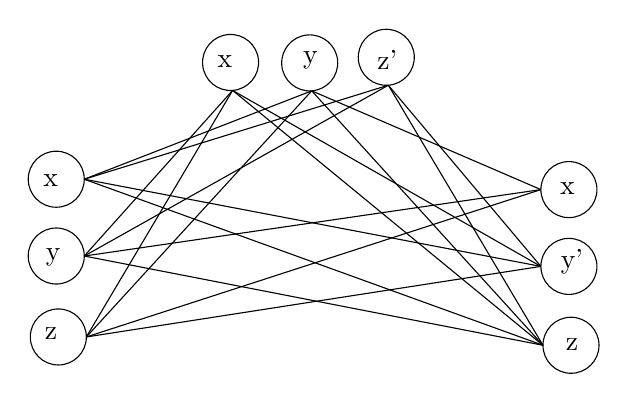
\begin{tikzpicture}[x=0.75pt,y=0.75pt,yscale=-1,xscale=1]
%uncomment if require: \path (0,300); %set diagram left start at 0, and has height of 300

%Shape: Circle [id:dp4939763876900307] 
\draw   (123,103.5) .. controls (123,96.04) and (129.04,90) .. (136.5,90) .. controls (143.96,90) and (150,96.04) .. (150,103.5) .. controls (150,110.96) and (143.96,117) .. (136.5,117) .. controls (129.04,117) and (123,110.96) .. (123,103.5) -- cycle ;
%Shape: Circle [id:dp5738913788864823] 
\draw   (123,140.5) .. controls (123,133.04) and (129.04,127) .. (136.5,127) .. controls (143.96,127) and (150,133.04) .. (150,140.5) .. controls (150,147.96) and (143.96,154) .. (136.5,154) .. controls (129.04,154) and (123,147.96) .. (123,140.5) -- cycle ;
%Shape: Circle [id:dp6688226687823849] 
\draw   (124,179.5) .. controls (124,172.04) and (130.04,166) .. (137.5,166) .. controls (144.96,166) and (151,172.04) .. (151,179.5) .. controls (151,186.96) and (144.96,193) .. (137.5,193) .. controls (130.04,193) and (124,186.96) .. (124,179.5) -- cycle ;
%Shape: Circle [id:dp4344206356699323] 
\draw   (370,108.5) .. controls (370,101.04) and (376.04,95) .. (383.5,95) .. controls (390.96,95) and (397,101.04) .. (397,108.5) .. controls (397,115.96) and (390.96,122) .. (383.5,122) .. controls (376.04,122) and (370,115.96) .. (370,108.5) -- cycle ;
%Shape: Circle [id:dp8247180711823536] 
\draw   (370,145.5) .. controls (370,138.04) and (376.04,132) .. (383.5,132) .. controls (390.96,132) and (397,138.04) .. (397,145.5) .. controls (397,152.96) and (390.96,159) .. (383.5,159) .. controls (376.04,159) and (370,152.96) .. (370,145.5) -- cycle ;
%Shape: Circle [id:dp8994586769064161] 
\draw   (371,183.5) .. controls (371,176.04) and (377.04,170) .. (384.5,170) .. controls (391.96,170) and (398,176.04) .. (398,183.5) .. controls (398,190.96) and (391.96,197) .. (384.5,197) .. controls (377.04,197) and (371,190.96) .. (371,183.5) -- cycle ;
%Shape: Circle [id:dp934018956755497] 
\draw   (294.52,31.29) .. controls (301.96,30.75) and (308.43,36.33) .. (308.97,43.77) .. controls (309.52,51.21) and (303.93,57.68) .. (296.5,58.22) .. controls (289.06,58.76) and (282.59,53.18) .. (282.05,45.74) .. controls (281.5,38.31) and (287.09,31.84) .. (294.52,31.29) -- cycle ;
%Shape: Circle [id:dp006234748608684559] 
\draw   (257.62,34) .. controls (265.06,33.45) and (271.53,39.04) .. (272.07,46.47) .. controls (272.62,53.91) and (267.03,60.38) .. (259.59,60.92) .. controls (252.16,61.47) and (245.69,55.88) .. (245.14,48.45) .. controls (244.6,41.01) and (250.19,34.54) .. (257.62,34) -- cycle ;
%Shape: Circle [id:dp1957125175145783] 
\draw   (219.5,33.78) .. controls (226.94,33.24) and (233.41,38.82) .. (233.95,46.26) .. controls (234.5,53.69) and (228.91,60.16) .. (221.48,60.71) .. controls (214.04,61.25) and (207.57,55.67) .. (207.03,48.23) .. controls (206.48,40.79) and (212.07,34.32) .. (219.5,33.78) -- cycle ;
%Straight Lines [id:da12954098064452435] 
\draw    (150,103.5) -- (259.59,60.92) ;


%Straight Lines [id:da4136075030434285] 
\draw    (150,103.5) -- (296.5,58.22) ;


%Straight Lines [id:da7316199944640691] 
\draw    (150,103.5) -- (371,183.5) ;


%Straight Lines [id:da6551763426736984] 
\draw    (150,103.5) -- (370,145.5) ;


%Straight Lines [id:da8387443114000026] 
\draw    (150,140.5) -- (371,183.5) ;


%Straight Lines [id:da21562488826992599] 
\draw    (150,140.5) -- (370,108.5) ;


%Straight Lines [id:da7242812945128725] 
\draw    (150,140.5) -- (296.5,58.22) ;


%Straight Lines [id:da826813214385727] 
\draw    (150,140.5) -- (221.48,60.71) ;


%Straight Lines [id:da8933302524547743] 
\draw    (151,179.5) -- (259.59,60.92) ;


%Straight Lines [id:da9305577911837748] 
\draw    (151,179.5) -- (221.48,60.71) ;


%Straight Lines [id:da5342783317932566] 
\draw    (151,179.5) -- (370,145.5) ;


%Straight Lines [id:da6551480872117615] 
\draw    (151,179.5) -- (370,108.5) ;


%Straight Lines [id:da8429593240550058] 
\draw    (221.48,60.71) -- (370,145.5) ;


%Straight Lines [id:da8436543998548214] 
\draw    (221.48,60.71) -- (371,183.5) ;


%Straight Lines [id:da5598554444333546] 
\draw    (296.5,58.22) -- (371,183.5) ;


%Straight Lines [id:da2028978494934136] 
\draw    (296.5,58.22) -- (370,145.5) ;


%Straight Lines [id:da5508883109065181] 
\draw    (259.59,60.92) -- (370,108.5) ;


%Straight Lines [id:da7317603843111179] 
\draw    (259.59,60.92) -- (371,183.5) ;



% Text Node
\draw (136,104) node  [align=left] {x };
% Text Node
\draw (135,141) node  [align=left] {y};
% Text Node
\draw (134,178) node  [align=left] {z};
% Text Node
\draw (296,46) node  [align=left] {z'};
% Text Node
\draw (385,183) node  [align=left] {z};
% Text Node
\draw (220,47) node  [align=left] {x };
% Text Node
\draw (385,108) node  [align=left] {x };
% Text Node
\draw (385,143) node  [align=left] {y'};
% Text Node
\draw (259,46) node  [align=left] {y};


\end{tikzpicture}

\end{center}
\subsection{Complexity Class}
We know that 3-SAT problem is NP-Complete. And since it can reduce to a clique problem in polynomial time, the clique problem is also $\mathcal{NP}$-complete.
\section{IND-SET problem}
\subsection{Definition}
A set of vertices from a graph that no two are adjacent.
\subsection{Definition II}
Given a graph $G$ and an integer $k$, does there exist a set of vertex whose size is larger or equal to $k$ s.t. all elements inside are non-adjacent.
\subsection{$\mathcal{NP}$}
To prove it is in $\mathcal{NP}$, we let the clue to be the set of vertex. Through linear search, we can check whether all vertices in the set are non-adjacent, this will lead to $\mathcal{O}(n^2)$ operations, which is polynomial time. 
\subsection{Graph construction}
The Graph is constructed as: 

Given the graph $G$ with $(V,E)$, let $G_1$ be the complete graph with $V$, and denote all edges from $G_1$ as $E_1$, the $G'$ is then defined as 
\[
	(V, E_1\backslash E)
\]
\subsection{Complexity Class}
Since we can reduce a `k-clique' problem into an `independent set problem' within polynomial operations, the independent set problem is also in $\mathcal{NP}$-complete complexity class.
\end{document}
